\documentclass[12pt]{article} % Set base font size to 12pt
\usepackage{graphicx}
\usepackage{geometry} % Adjust page margins
\usepackage{setspace} % Line spacing
\usepackage{titlesec} % Customize section titles
\usepackage{tocloft} % Customize table of contents
\usepackage{fancyhdr} % Headers and footers
\usepackage{hyperref} % Add hyperlinks
\usepackage{xcolor} % Color package

% Set page margins
\geometry{a4paper, margin=2.5cm}

% Set line spacing
\setstretch{1.5} % Adjust line spacing for better readability

% Customize section titles
\titleformat{\section}[block]{\LARGE\bfseries\color{black}}{}{0em}{\filcenter}
\titlespacing*{\section}{0pt}{3.5ex plus 1ex minus .2ex}{2.3ex plus .2ex}

% Customize table of contents
\renewcommand{\cftsecleader}{\cftdotfill{\cftdotsep}}
\renewcommand{\contentsname}{Inhaltsverzeichnis}
\renewcommand{\cftaftertoctitle}{\par\nobreak\bigskip\bigskip\bigskip} % Add space after TOC title
\setlength{\cftbeforesecskip}{0.5em} % Adjust spacing between section entries
\setlength{\cftaftertoctitleskip}{2cm} % Adjust spacing between TOC title and entries
\hypersetup{
    colorlinks=true,
    linkcolor=blue,
    filecolor=magenta,
    urlcolor=cyan,
}

% Define headers and footers
\pagestyle{fancy}
\fancyhf{} % Clear default headers and footers
\fancyhead[R]{\thepage} % Page number on right side of header
\fancyhead[L]{\nouppercase{\leftmark}} % Chapter title on left side of header
\renewcommand{\headrulewidth}{0pt} % Remove header line
\fancyfoot[C]{\thepage} % Page number in the center of footer
\renewcommand{\footrulewidth}{0pt} % Remove footer line

% Define light gray color
\definecolor{lightgray}{RGB}{240,240,240}

\begin{document}

% Title Page
\begin{titlepage}
    \centering
    \vspace*{3cm}
    {\Huge\bfseries\textcolor{blue}{\MakeUppercase{ Whispers of the Moon }}\par} % Increased font size and colored title
    \vspace{0.5cm} % Adjust space between title and author
    {\Large\textit{ Maja Schmidt }\par} % Italic author name
    \vfill
    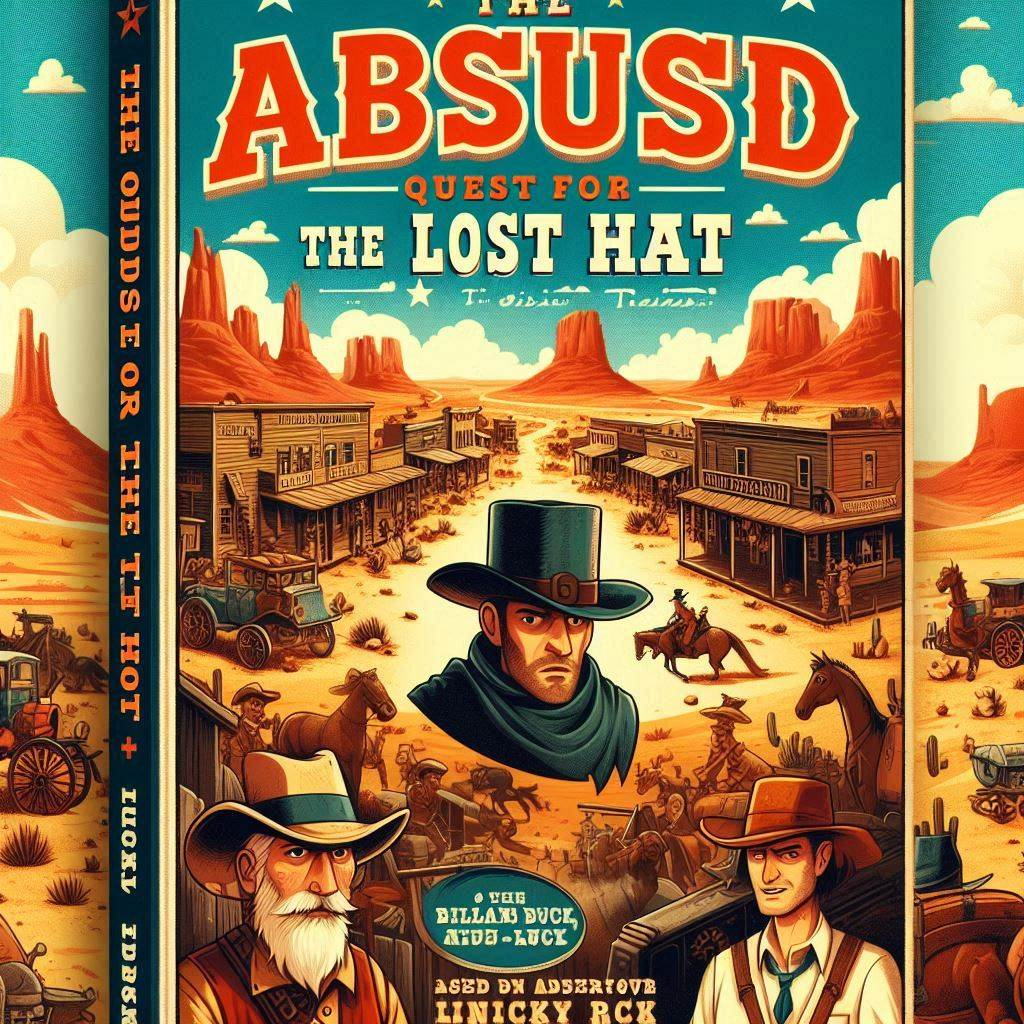
\includegraphics[width=0.9\textwidth]{ cover.jpg } % Larger cover image
    \vfill
    \today
\end{titlepage}

% Autorenvita
\section*{Autorenvita}
\vspace{4cm} % Adjust space between "Autorenvita" and "Inhaltsverzeichnis"
\begin{minipage}{\textwidth}
    Maja Schmidt ist eine renommierte Autorin, die sich auf romantische Geschichten mit kulturellen und atmosphärischen Elementen spezialisiert hat. Mit einer Leidenschaft für die asiatische Kultur und Kunst hat sie bereits mehrere erfolgreiche Bücher veröffentlicht, die Leser auf fesselnde Reisen durch die Liebe und kulturelle Vielfalt entführt haben.
\end{minipage}

% Place table of contents on a separate page
\clearpage
\tableofcontents
\clearpage

% Chapters

\section{ Begegnung unter dem Mond }
\begin{minipage}{\textwidth}
    Mei war fasziniert von den kunstvollen Gemälden, die in der Ausstellung präsentiert wurden. Als sie sich umdrehte, um das Bild eines traditionellen chinesischen Gartens zu betrachten, bemerkte sie einen gut gekleideten Mann, der sie mit einem warmen Lächeln ansah. Es war Leo, der charmante Galerist, der die Ausstellung organisiert hatte. Sie spürte eine unerklärliche Verbindung zu ihm, als ihre Blicke sich trafen. 'Guten Abend, Mei', begrüßte Leo sie mit sanfter Stimme. 'Guten Abend, Leo', erwiderte Mei leicht errötend. Sie führten angeregte Gespräche über die Kunstwerke und die chinesische Kultur. Die Zeit verging wie im Flug, und bevor sie es bemerkten, war die Ausstellung zu Ende. Leo schlug vor, dass sie gemeinsam einen Spaziergang durch die malerischen Gassen von Shanghai machen sollten. Unter dem klaren Mondlicht begann ihre romantische Reise, die voller Geheimnisse und unerwarteter Enthüllungen sein sollte.
\end{minipage}

\section{ Verborgene Schätze }
\begin{minipage}{\textwidth}
    Mei und Leo schlenderten Hand in Hand durch die malerischen Gassen von Shanghai, die von traditionellen chinesischen Laternen beleuchtet wurden. Die Atmosphäre war magisch, und Mei fühlte sich, als würde sie in eine andere Zeit eintauchen. Leo erzählte ihr faszinierende Geschichten über die verborgenen Schätze der chinesischen Kultur, die in den engen Gassen und versteckten Höfen zu finden waren. Mei lauschte gebannt seinen Worten und spürte, wie ihr Verständnis für ihre eigene Kultur und Geschichte wuchs. Plötzlich blieb Leo vor einer alten, verzierten Tür stehen und lud Mei ein, mit ihm einzutreten. Hinter der Tür verbarg sich ein atemberaubender chinesischer Garten, der von kunstvollen Statuen und blühenden Bäumen geschmückt war. 'Das ist einer der verborgenen Schätze, von denen ich dir erzählt habe', sagte Leo mit einem geheimnisvollen Lächeln. Während sie den Garten erkundeten, kamen sie an einem antiken Artefakt vorbei, das Meis Aufmerksamkeit erregte. Leo erklärte ihr die Bedeutung und die Geschichte des Artefakts, und plötzlich fühlte Mei, wie sich die ersten Geheimnisse um sie herum zu entwirren begannen. Es war, als ob der Garten und seine Schätze ihr eine Botschaft über ihre eigene Vergangenheit übermitteln wollten. Die Nacht verging, und Mei und Leo kehrten mit einem Gefühl der Ehrfurcht und Neugierde in ihre Welt zurück, bereit, die Geheimnisse, die sich vor ihnen auftaten, zu erkunden.
\end{minipage}

\section{ Geheimnisse der Vergangenheit }
\begin{minipage}{\textwidth}
    Mei und Leo standen in einem alten chinesischen Garten, umgeben von duftenden Blumen und dem sanften Plätschern eines Teiches. Die Enthüllung von Meis Vergangenheit hatte eine unerwartete Wendung genommen und ihre Liebe wurde auf die Probe gestellt. Leo sah sie mitfühlend an und legte sanft seine Hand auf ihre Schulter. 'Mei, ich bin hier, um dich zu unterstützen, egal was passiert', versicherte er ihr. Mei kämpfte mit ihren Emotionen, während sie die Wahrheit über ihre Familie und ihre Wurzeln verarbeitete. 'Leo, ich weiß nicht, ob ich stark genug bin, um damit umzugehen', gestand sie mit zitternder Stimme. In diesem Moment trat Nan, Meis treue Freundin, aus dem Schatten hervor. 'Mei, du bist stärker, als du denkst. Wir werden das gemeinsam durchstehen', ermutigte sie sie. Gemeinsam begannen sie, die Geheimnisse der Vergangenheit zu entwirren und stießen auf Hinweise, die sie zu einem alten chinesischen Artefakt führten. Die Entscheidungen, die sie treffen mussten, würden ihr Schicksal für immer verändern. Inmitten der Geheimnisse und der emotionalen Turbulenzen fanden sie jedoch auch Trost und Unterstützung in ihrer unerschütterlichen Freundschaft.
\end{minipage}

\section{ Entscheidungen im Mondschein }
\begin{minipage}{\textwidth}
    Die klaren Strahlen des Monds beleuchteten die malerischen Gassen von Shanghai, als Mei und Leo sich an einem ruhigen Ort niederließen, um über die Enthüllungen der vergangenen Tage zu sprechen. Mei fühlte sich von den Geheimnissen ihrer eigenen Geschichte überwältigt, und Leo war fest entschlossen, sie in dieser schwierigen Zeit zu unterstützen. 'Mei, ich weiß, dass die Enthüllungen über deine Vergangenheit überwältigend sind, aber du bist stark genug, um damit umzugehen', sagte Leo sanft und legte seine Hand auf Meis, um sie zu trösten. Mei sah ihn mit Tränen in den Augen an und spürte die tiefe Verbundenheit, die zwischen ihnen gewachsen war. 'Danke, Leo. Deine Unterstützung bedeutet mir alles', flüsterte sie. In diesem Moment wusste Mei, dass sie sich auf Leo verlassen konnte, egal was die Zukunft bringen mochte. Doch sie standen vor schwierigen Entscheidungen, die ihr Leben für immer verändern würden. Nan, Meis treue Freundin, trat zu ihnen und reichte Mei einen Brief. 'Mei, ich habe etwas entdeckt, das deine Vergangenheit noch weiter erhellen könnte', sagte Nan aufgeregt. Mei öffnete den Brief und las die Worte, die ihr eine neue Perspektive auf ihr Leben boten. Die Entscheidungen, die sie nun treffen musste, waren von großer Tragweite. Doch mit der Unterstützung von Leo und Nan fühlte sie sich bereit, den Geheimnissen ihrer Vergangenheit ins Auge zu blicken und die Weichen für ihre Zukunft zu stellen. Unter dem sanften Mondschein trafen Mei und Leo schwierige Entscheidungen, die ihr Schicksal für immer verändern sollten.
\end{minipage}

\clearpage
% Metadata
\section*{Metadaten}
\begin{minipage}{\textwidth}
    \colorbox{lightgray}{
        \begin{minipage}{\dimexpr\textwidth-2\fboxsep}
            \vspace{4cm}
            \begin{itemize}
                \item Name des Buches: Whispers of the Moon
                \item Name des Autors: Maja Schmidt
                \item Name des Herausgebers: Mark Zimmermann
                \item Name des Verlags: HdM AI Technologies
                \item Adresse des Verlags: Nobelstraße 10, 70569 Stuttgart
                \item Datum der Veröffentlichung: 2022-10-20
            \end{itemize}
            \vspace{4cm}
        \end{minipage}

    }
\end{minipage}


\end{document}